\section{Statistical Generation as Planning}
\label{sec:pcrisp}

We now extend \crisp\ to statistical generation (\pcrisp). The basic idea is to add a statistical grammar model while leaving the sentence generation mechanism untouched. This way we can select the highest scoring derivation which satisfies all constraints (grammaticality, expresses the communicative goal, uses unambiguous referring expressions, etc.). 

 As a straightforward probability model over {\sc ltag} derivations we choose probabilistic {\sc tag} ({\sc ptag}) \cite{resnik1992}.
Our choice of {\sc ptag} for sentence generation is motivated by a number of attractive properties.
 {\sc Ptag} is lexicalized and therefore does not only assign probabilities to operations in the grammar (as for example plain {\sc pcfg}), but also accounts for binary dependencies between words.  Unlike n-gram models however, these co-occurrences are structured according to local syntactic context as a result of {\sc tag}'s extended domain of locality. The probability model describes how the syntactic arguments of a word are typically filled. 
Furthermore, as {\sc tag} factors recursion from the domain of dependencies, the probability for core constructions remains the same independent of additional adjunctions. 
%Second, {\sc ptag} is a generative model. This is crucial because it allows us to assign probabilities to partial derivations. In addition we use the probability of partial derivations as a cost function, to help guide search through the space of possible PLTAG derivations. In contrast, other statistical generation systems use discriminative models that select the best possible generation output from a set of candidate sentences.
%Finally, the independence assumption makes it easy to estimate {\sc ptag}s from a treebank.
 We review {\sc ptag} in section \ref{ssec:probmodels}.

While we leave the basic sentence generation mechanism intact, we need to modify the concrete formulation of \crisp\ planning operators to accommodate bilexical dependencies. Likewise, we need to take the step from classical planning to \emph{metric} planning systems which can use the probabilities.
In metric planning \cite{fox2002}, planning actions can modify the value of numeric variables in addition to adding and deleting logical literals to the state. The goal state specifies constraints on this variable. In the simplest case the variable can only be increased by a static cost value in each action, and the goal state contains the objective to minimize the total cost. While systems such as Metric-{\sc FF} \cite{hoffmann2003} do not guarantee optimality, they do generally offer good results. We address our encoding of sentence generation with {\sc ptag} as metric planning in section \ref{ssec:pcrisp-domains}. 

\subsection{Probabilistic TAG}
\label{ssec:probmodels}
{\sc ptag} \cite{resnik1992} views {\sc tag} derivations as sequences of events of three types: initial events, substitution events, and adjunction events.

The probability distribution for initial events describes how likely it is to start any derivation with a given initial tree. 
It is defined over all initial trees $\alpha \in I$ with their possible lexicalizations $w \in W_\alpha$: 
$$ \sum\limits_{\alpha \in I}\sum\limits_{w \in W_\alpha} P_i(\init(\alpha, w)) = 1 $$

For substitution events, there is a probability distribution for each substitution node $n$ of each elementary tree $\tau$ lexicalized with $v$, which describes how likely it is to substitute it with an initial tree $\alpha$ lexicalized with $w$. 
$$\sum\limits_{\alpha \in I}\sum\limits_{w \in W_\alpha} P_s(\subst(\tau,v , \alpha, w, n)) = 1$$

Similarly for each internal node there is a distribution that describes the probability to adjoin an auxiliary tree $\beta \in A$ lexicalized with $w$. In addition some probability mass is reserved for the event of not adjoining anything to such a node at all.

$$ P_a(\noadj(\tau, v, n)) + \strut$$
$$ \sum\limits_{\beta \in A}\sum\limits_{w \in W_\beta} P_a(\adj(\tau, v, \beta, w, n)) = 1.$$

{\sc Ptag} assumes that all events occur independently of each other. Therefore it defines the total probability for a derivation as the product of the probability of its individual events. 

\subsection{PCRISP Planning Domains}
\label{ssec:pcrisp-domains}
Using the definition of {\sc ptag}, we now reformulate the \crisp\ planning operators described in section \ref{ssec:crispdomain}.
The independence assumption in {\sc ptag} allows us to continue to model each addition of a single elementary tree to the derivation (with a certain probability score). However, while \crisp\ planning operators can add an elementary tree to any site of the correct category, {\sc ptag} substitution and adjunction events are binary events between lexicalized trees at a specific node. We therefore adapt the literals that record open substitution and adjunction sites in partial derivations accordingly and create one operator for each node in each possible combination of lexicalized trees.
Fig.~\ref{example-action} shows an example planning operator for each type.
\begin{figure}[t]
\begin{center}
\cplanaction{\bf subst-t3-cat-t28-eats-n1(u,~x1)}{referent(u,~x1),\\ subst(t28-eats,~n1,~u), cat(x1)}{
$\lnot$needtoexpr(pred-cat,~x1),\\ $\lnot$subst(t-28-eats, n1,~u),\\
adj(t3-cat, n2 u)}{4.3012}\\\smallskip

\cplanaction{\bf adj-t5-raw-t3-fish-n2(u,~x1)}{referent(u,~x1),\\ adj(t28-eats,n2,~u), raw(x1)}{
$\lnot$needtoexpr(pred-raw,~x1),\\ $\lnot$adj(t-28-eats, n2,~u)}{6.9076}\\\smallskip

\cplanaction{\bf init-t28-eats(u,~x1,~x2,~x3)}{referent(u,~x1),\\ eats(x1,~x2,~x3)}{
$\lnot$needtoexpr(pred-eats,~x1,~x2,~x3), \\
 subst(t-28-eats,~n1,subj), subst(t28-eats,~n4,obj),\\
adj(t-28-eats, n2, u), adj(t-28-eats, n3, u)}{8.5172}\\\smallskip

\cplanaction{\bf noadj-t28-eats-n3(u)}{
 adj(t-28-eats,~n3,u)}
{$\lnot$ adj(t-28-eats, n3, u)}{0.1054}\\\smallskip

\caption{\label{example-action} Some \pcrisp\ operators for the grammar from Fig.~\ref{fig:grammar}.}
\end{center}
\end{figure}

Finally, we set the cost of an operator to be its negative log probability. For example 
\begin{align*}
&Cost(\mbox{subst-t3-cat-t28-eats-n1}) = \\
 & \qquad -\log P_s(\subst(\mathrm{t3},\textit{`cat'},\mathrm{t28},\textit{`eats'},\mathrm{n1})) ).
\end{align*}
This way the plan which minimizes the sum of the costs of its actions  corresponds to the {\sc tag} derivation with the highest probability. 

\subsection{Dealing with Data Sparseness}
\label{ssec:sparseness}
The event definition of {\sc ptag} is very-fine grained. Substitution and adjunction events depend on specific parent and child trees with specific lexicalizations and on a node in the parent tree, as illustrated in Fig.~\ref{fig:modelillustration}, B.1. When we estimate a probability model from training data, we cannot expect to observe evidence for all combinations of trees. Derivations that include such unseen events have zero probability and are therefore impossible. As we show in section \ref{sec:experiments}, this gives rise to a massive data sparseness problem.

  A straightforward way to deal with data sparseness is to drop all lexicalizations from event definitions, as illustrated in Fig.~\ref{fig:modelillustration}, A. Unfortunately this model  no longer accounts for bilexical dependencies between words. Since our system has to add a lexicalized tree in each step, lexicalizations for this child tree should always be taken into account by the probability model, if available. Despite these drawbacks, we perform experiments with the unlexicalized model as a baseline. This allows us to investigate if purely syntactic information is sufficient to achieve high quality generation output.

An alternative model computes linear interpolation between three back-off levels. The first level is just standard {\sc ptag} (Fig.~\ref{fig:modelillustration}, B.1), for the second level the lexicalizations of the parent tree is dropped (Fig.~\ref{fig:modelillustration}, B.2), for the third level the model describes only the distribution of lexicalized child trees over each category (Fig.~\ref{fig:modelillustration}, B.3).  
Notice also that the third level is similar in spirit to a probabilistic version of original \crisp\ operators (compare Fig.~\ref{fig:modelillustration}, B.3 and Fig.~\ref{fig:crisp-operators}). 
\begin{figure}[t]
\begin{center}
\includegraphics[width=.5\textwidth]{figures/modelillustration}
\caption{\label{fig:modelillustration} Illustration of the unlexicalized probability model (A) and the three back-off levels of the linear interpolation model (B).}

\end{center}
\end{figure}


%It is obvious that the number of total planning operators grows quadratically with the number of possible input words in the grammar. In practice this causes a problem for most heuristic search planners, which will instantiate planning operators to all possible actions before attempting to solve the problem. Our generation system therefore only selects operators that are compatible with the input semantics before running the planner. 
%On the other hand,


%\newcommand{\init}[0]{\textit{ init}}
%\newcommand{\subst}[0]{\textit{ subst}}

%\begin{figure}[p]
%\caption{\label{modelillustration} The three back-off levels.}
%\begin{center}
%\includegraphics[width=.5\textwidth]{modelillustration}
%\end{center}
%\end{figure}





%%% Local Variables:  %%% mode: latex %%% TeX-master: "pcrisp-10" %%% End: 